\documentclass{article}
\usepackage{amsmath}
\usepackage{graphicx}
\usepackage[utf8]{inputenc}

\title{Assignment 1}
\author{D V K M Rishab, AI20MTECH14004 }
\date{September 2, 2020}

\begin{document}

\maketitle

\section*{Assignment 1}
 Solution: 
 \newline \newline
 \begin{math}
 Vector, P = \begin{pmatrix} 7 \\ 6 \\ \end{pmatrix} \newline \newline \newline
 Vector, Q = \begin{pmatrix} 3 \\ 4 \\ \end{pmatrix} \newline \newline \newline
 A point on the X-axis is equidistant to both P and Q. \newline \newline
 Need to find x. \newline \newline
 \implies 
 \left\lVert \begin{pmatrix} x \\ 0 \\ \end{pmatrix} - \begin{pmatrix} 7 \\ 6 \\ \end{pmatrix} \right\rVert^2 = \left\lVert \begin{pmatrix} x \\ 0 \\ \end{pmatrix} - \begin{pmatrix} 3 \\ 4 \\ \end{pmatrix} \right\rVert^2 \newline \newline \newline \newline
 \implies 
 \left\lVert  x \right\rVert^2 + \left\lVert\begin{pmatrix} 7 \\ 6 \\ \end{pmatrix} \right\rVert^2 - 2\begin{pmatrix} 7 & 6 \end{pmatrix}\begin{pmatrix} x \\ 0 \\ \end{pmatrix} = \left\lVert  x \right\rVert^2 + \left\lVert\begin{pmatrix} 3 \\ 4 \\ \end{pmatrix} \right\rVert^2 - 2\begin{pmatrix} 3 & 4 \end{pmatrix}\begin{pmatrix} x \\ 0 \\ \end{pmatrix}  \newline \newline \newline
 \implies 7^2 +6^2 - 2\begin{pmatrix} 7 & 6 \end{pmatrix}\begin{pmatrix} x \\ 0 \\ \end{pmatrix}  = 3^2 + 4^2 - 2\begin{pmatrix} 3 & 4 \end{pmatrix}\begin{pmatrix} x \\ 0 \\ \end{pmatrix} \newline \newline
 \implies 85 - 2\begin{pmatrix} 7 & 6 \end{pmatrix}\begin{pmatrix} x \\ 0 \\ \end{pmatrix} = 25 - 2\begin{pmatrix} 3 & 4 \end{pmatrix}\begin{pmatrix} x \\ 0 \\ \end{pmatrix} \newline \newline
 \implies 60 = \begin{pmatrix} 8 & 4 \end{pmatrix}\begin{pmatrix} x \\ 0 \\ \end{pmatrix} \newline \newline
 \implies 8x = 60 \newline \newline
 \implies x = 15/2 \newline \newline
 Therefore, \hspace{0.1cm} the \hspace{0.1cm} vector \hspace{0.1cm} equidistant \hspace{0.1cm} to \hspace{0.1cm} both \hspace{0.1cm} P \hspace{0.1cm} and \hspace{0.1cm} Q \hspace{0.1cm} is \hspace{0.1cm} \begin{pmatrix} 15/2 \\ 0 \\ \end{pmatrix}
 \end{math}
\begin{figure}
\centering
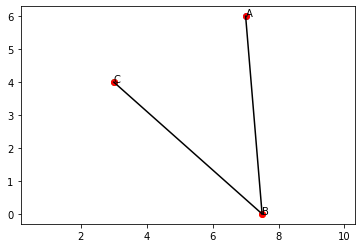
\includegraphics{Plot.png}
\caption{Plot representing the Points}
\label{Fig.1}
\end{figure}
\end{document}
